\chapter{Volba technologií a návrh architektury}

Pro tento projekt je potřeba zvolit dvě technologie, první pro vývoj samotného rozšíření do webových prohlížečů a druhou pro vývoj podpůrného serveru. Pro webové rozšíření bylo potřeba zvolit technologii, která umožňuje kompilaci nebo transpilaci do jazyka JavaScript, protože to je jediný programovací jazyk, který je podporován v~běhovém prostředí webových prohlížečů.

\section{Volba technologie pro webové rozšíření}

Jak již bylo zmíněno v~předchozím odstavci, hlavním požadavkem na technologii zvolenou pro vývoj rozšíření do webových prohlížečů je zvolit programovací jazyk, který umožňuje transpilaci do jazyka JavaScript. Transpilace je proces, při kterém dochází k~překladu zdrojových kódů z~původního programovacího jazyka do syntetizovaného kódu v~cílovém jazyce \cite{fowler_transparent_2013}. 

Je poměrně časté, že v~procesu transpilace je zdrojový a cílový jazyk stejný programovací jazyk, ale jedná se o~jinou verzi tohoto jazyka. Typickým důvodem pro takovou transpilaci je zachování zpětné kompatibility se staršími verzemi daného programovacího jazyka. Pomocí této transpilace je možné používat například moderní syntaxi a jazykové konstrukce, které byly přidané až v~novější verzi tohoto programovacího jazyka, bez dopadu na míru podpory těchto přidaných konstrukcí v~běhovém prostředí.

\subsection{Výčet některých z~dostupných technologií}

Pro implementaci rozšíření do webového prohlížeče se naskytuje několik programovacích jazyků, které splňují vymezené požadavky na kompatibilitu s~běhovým prostředím internetových prohlížečů:

\begin{itemize}
    \item JavaScript
    \item TypeScript
    \item Kotlin/JS
    \item Ostatní programovací jazyky s~podporou transpilace do jazyka JavaScript
\end{itemize}

Pro každý z~těchto programovacích jazyků existuje řada pro a proti, které je potřeba při výběru zvážit. V~následujících odstavcích je stručně představena každá z~variant společně s~výhodami a nevýhodami daného programovacího jazyka.

\subsubsection{JavaScript}

 Programovací jazyk JavaScript je implementací specifikace jazyka ECMAScript a jedná se v~dnešní době o~jeden z~nejrozšířenějších jazyků vůbec. Bezesporu největší výhodou tohoto jazyka je, že je přímo podporovaný v~běhovém prostředí webových prohlížečích, a není tedy potřeba zavádět žádný další krok pro sestavení kódu rozšíření \cite[kap. 1]{flanagan_javascript_2020}\footnote{Autorem všech překladů z~angličtiny je autor práce}. 
 Nevýhodou programovacího jazyka JavaScript je, že se jedná o~dynamicky typovaný programovací jazyk. To znamená, že datové typy proměnných se vyhodnocují až za běhu programu, a je tedy mnohem jednodušší udělat při psaní programu chybu v~porovnání s~programovacími jazyky, které jsou staticky typované. Staticky typované programovací jazyky jsou takové jazyky, u~kterých je datový typ všech proměnných znám již při překladu programu \cite[kap. 3.1]{flanagan_javascript_2020}.

\subsubsection{TypeScript}

Programovací jazyk TypeScript je z~pohledu syntaxe striktní nadmnožinou programovacího jazyka JavaScript. 
To implikuje, že jakýkoliv syntakticky validní program napsaný v~jazyce JavaScript je zároveň syntakticky validním programem v~jazyce TypeScript. Zmíněná implikace však neplatí opačným směrem, protože TypeScript rozšiřuje JavaScript o~novou syntaxi a jazykové konstrukce, které nejsou v~jazyce JavaScript nativně podporovány \cite{cherny_programming_2019}

Nejzásadnější přidanou hodnotou jazyka TypeScript, jak již název naznačuje, je podpora pro typový systém, který tento programovací jazyk zařazuje mezi staticky typované programovací jazyky, protože všechny datové typy jsou předem známy již při překladu programu. 

Ve výpisech \ref{code:javascript-bad} a \ref{code:typescript-good} je vidět porovnání programovacích jazyků JavaScript a Typescript společně s~nastíněním výhod, které přináší využití programovacího jazyka TypeScript.

\begin{lstlisting}[label={code:javascript-bad}, caption={Ukázka kódu s~neplatným typem parametru v~jazyce JavaScript (vlastní zpracování)}]
// JavaScript
function format(price) {
    return price.toFixed(2);
}

format(2.134); // -> '2.13'
format("2.134"); // Způsobí chybu až při spuštění programu
// Uncaught TypeError: price.toFixed is not a function
\end{lstlisting}

\begin{lstlisting}[label={code:typescript-good}, caption={Ukázka kódu s~neplatným typem parametru v~jazyce TypeScript (vlastní zpracování)}]
// TypeScript
function format(price: number): string {
    return price.toFixed(2);
}

format(2.134); // -> '2.13'
format("2.134"); // Způsobí chybu při kompilaci, ještě před spuštěním
// Argument of type 'string' is not assignable to parameter of type 'number'.
\end{lstlisting}

Výhodou jazyka TypeScript je interoperabilita s~jazykem JavaScript, která umožňuje z~jazyka TypeScript využívat softwarové knihovny napsané v~jazyce JavaScript, včetně již zmíněného API poskytovaného běhovým prostředím webového prohlížeče. Pro tyto knihovny a API často existují typové definice, což jsou speciální soubory, které obsahují externí deklaraci typů pro existující JavaScript knihovny. Tyto typové definice je možné nainstalovat spolu s~ostatními závislostmi programu. Například typové definice pro API běhového prostředí Node.js jsou dostupné v~podobě NPM (Node Package Manager) balíčku \verb|@types/node| \cite[kap. 2]{cherny_programming_2019}.

Nevýhodou jazyka TypeScript je, že webové prohlížeče neumí na rozdíl od jazyka JavaScript kód v~jazyce TypeScript nativně interpretovat a proto je nutné před spuštěním celý program transpilovat do jazyka JavaScript, který odstraní typové definice a ostatní přidané syntaktické a jazykové konstrukce, které nejsou součástí specifikace ECMAScript. 

\subsubsection{Kotlin/JS}\label{sec:kotlin}

Kotlin je programovací jazyk vyvinutý společností JetBrains s.r.o., která se specializuje v~oblasti vývoje programovacích nástrojů a vývojových prostředí. Jedná se o~programovací jazyk, který je možné zkompilovat do několika cílových výstupních formátů. Dominantním cílem kompilace pro jazyk Kotlin je JVM bytecode, což je nativní kód pro prostředí Java Virtual Machine. Programovací jazyk Kotlin umožňuje mimo jiné i kompilaci do nativního strojového kódu pomocí Kotlin native s~vazbami na nástroj LVVM (Low Level Virtual Machine) a transpilaci do jazyka JavaScript pomocí platformy Kotlin/JS.

Stejně jako u~programovacího jazyka TypeScript, programovací jazyk Kotlin nabízí interoperabilitu s~již existujícími JavaScript knihovnami, která je zprostředkovaná pomocí typových deklarací a anotací. 
U~JavaScript knihoven, které se distribují společně s~typovými definicemi jazyka TypeScript je možné využít nástroj Dukat, který automaticky konvertuje typové definice jazyka TypeScript do typových definic jazyka Kotlin. Alternativou je manuální definice těchto typových definic.

V~jazyce Kotlin k~tomuto účelu slouží klíčové slovo \code{external}, které definuje objekty, funkce, třídy a další entity z~externích knihoven. Výpisy \ref{code:kotlin-js-javascript} a \ref{code:kotlin-js-typedefs} zobrazují implementaci jednoduché softwarové knihovny v~programovacím jazyce JavaScript a k~ní přidružené typové definice v~programovacím jazyce Kotlin.

\begin{lstlisting}[label={code:kotlin-js-javascript}, caption={Jednoduchá JavaScript knihovna pro demonstraci typových definic v~jazyce Kotlin (vlastní zpracování)}]
// library.js
const square = (x) => x * x;

function add(x, y) {
    return x + y;
}

class Node {
    constructor(x) {
        this.x = x; 
    }
}
\end{lstlisting}

\begin{lstlisting}[label={code:kotlin-js-typedefs}, caption={Typové definice v~jazyce Kotlin pro externí JavaScript knihovnu (vlastní zpracování)}]
// typedef.kt
external val square: (Int) => Int
external fun add(x: Int, y: Int): Int
external class Node(val x: Int)
\end{lstlisting}

Kotlin/JS přináší několik výhod. První, subjektivní výhodou pro tento konkrétní projekt je, že s~tímto programovacím jazykem má autor již dlouholetou zkušenost. Mezi další, již více objektivní, výhody patří mimo jiné typový systém jazyka Kotlin, který přináší zlepšení oproti typovému systému, který implementuje programovací jazyk TypeScript. Příkladem zlepšení může být rozlišení datových typů pro celočíselná a desetinná čísla v~různých bitových velikostech. Další z~výhod je rozsáhlejší standardní knihovna programovacího jazyka Kotlin, kterou je možné přímo v~rámci programu využívat. 

Potencionální výhodou by v~případě, že by tento programovací jazyk byl zvolen pro implementaci webového rozšíření, byly již existující vazby a typové definice pro populární knihovnu React.js, které spravuje přímo firma JetBrains s.r.o., což zaručuje kvalitu typových definic a lepší komerční i nekomerční podporu než u~knihoven, které vyvíjí jeden člověk,  a to navíc často ve svém volném čase.

Hlavní nevýhodou použití jazyka Kotlin je náročný proces kompilace, který vyžaduje celou řadu externích nástrojů. Další nevýhodou tohoto programovacího jazyka je, že v~době psaní této práce neexistuje typová definice pro velice obsáhlé aplikační rozhraní webových prohlížečů, která by musela být nadefinována v~rámci projektu, což by bylo velice složité a časově náročné, protože prohlížeče pracují s~rozšířenou sadou objektů oproti běhovému prostředí pro aplikace webových stránek, pro které je Kotlin/JS primárně určen.

\subsubsection{Ostatní programovací jazyky s~podporou transpilace do jazyka JavaScript}

Existuje celá řada dalších programovacích jazyků, které podporují transpilaci do jazyka JavaScript. Jedná se například programovací jazyk Scala, Clojure, PureScript, CofeeScript, Dart, ReasonML nebo Haxe.

Žádný z~těchto jazyků ale nepřináší v~kontextu webových rozšíření zásadní objektivní výhody oproti již zmíněným programovacích jazykům a jedná se často pouze o~preferenci syntaxe daného jazyka. Tyto jazyky byly vyřazeny z~výběru mimo jiné i kvůli nedostatečné zkušenosti autora s~jejich používáním.  

\subsection{Zvolená technologie}

Po zvážení výhod a nevýhod zmíněných jazyků byl pro implementaci rozšíření zvolen programovací jazyk TypeScript, protože nabízí nejlepší kompromis mezi rychlostí vývoje a kvalitou výsledného kódu. Sestavování transpilovaného výstupu v~jazyce JavaScript je v~případě využití programovacího jazyka TypeScript přímočaré a kompilátor pro překlad TypeScript kódu je možné spouštět velice často, bez delších časových prodlev. Rychlost transpilace se pohybuje u~menších projektů maximálně v~jednotkách sekund, častěji spíše v~desítkách až stovkách milisekund. V~porovnání například se zmíněnou technologií Kotlin/JS jde o~výraznou redukci kompilačního času, protože transpilace z~jazyka Kotlin do jazyka JavaScript přes nástroj Gradle může trvat až několik minut, což se může velice negativně projevit na produktivitě při vývoji rozšíření.

\section{Volba technologie pro podpůrný webový server}

Pro podpůrný webový server se nabízí daleko širší spektrum technologií, ze kterých je možné pro implementaci programu vybírat. Tato diverzita je dána mimo jiné tím, že na podpůrný webový serveru není kladeno omezení na kompatibilitu s~konkrétním běhovým prostředím, jako je tomu u~rozšíření do webových prohlížečů. 

\subsection{Požadavky na zvolenou technologii}\label{sec:pozadavky-na-zvolenou-technologii}

Vybraný programovací jazyk a webový aplikační rámec musí podporovat následující požadavky na vestavěné funkcionality, aby bylo možné tento rámec pro implementaci podpůrného webového serveru použít:

\begin{itemize}
    \item Přijímání a odpovídání na přijaté HTTP požadavky,
    \item serializace a parsování formát JSON pro přenos dat,
    \item komunikace s~databází, ve které jsou uložená data uživatelů,
    \item podpora pro autentikaci a autorizaci uživatelů s~využitím HTTP hlaviček,
    \item odesílání emailů pomocí vestavěného nebo externího SMTP serveru.
\end{itemize}

Tyto požadavky splňuje množství aplikačních rámců napříč širokou škálou programovacích jazyků. Toto spektrum technologií bylo zúženo na 4 konkrétní aplikační rámce, které budou popsány v~následujících podkapitolách.

\subsection{Představení dostupných technologií}

\subsubsection{Spring framework}\label{sec:spring-boot}

% https://spring.io/

Spring Framework a jeho nadstavba Spring Boot je aplikační rámec vyvinutý společností Pivotal v~roce 2004 \cite{risberg_spring_2004}, která je od roku 2019 součást společnosti VMware \cite{vmware_pivotal_acquisition_2019}. Jedná se o~open source aplikační rámec, který staví na technologii programovacího jazyka Java a je proto možné pro vývoj aplikací v~tomto aplikačním rámci použít libovolný programovací jazyk, který je kompatibilní s~běhovým prostředím Java Virtual Machine. Oficiálně podporovanými programovacími jazyky jsou Java, Kotlin a Groovy \cite{spring_framework}.

Spring nabízí řadu modulů, které je možné využít při programování aplikací. Tyto moduly jsou dostupné jako samostatné balíčky a je možné je specifikovat v~rámci závislostí v~nástroji pro sestavování balíčků jako je například Maven nebo Gradle. Tato modularita nabízí flexibilitu při vývoji aplikací, kdy nedochází ke stahování, kompilaci a exportu softwarových knihoven, které nejsou pro konkrétní aplikaci potřeba. Příkladem může být modul \code{spring-data}, který poskytuje sdílenou logiku a abstrakce pro načítání dat z~relačních a NoSQL databází. Pokud aplikace nepotřebuje ukládat data v~databázi a místo toho data získává například z~externího REAST API, není potřeba tento modul do aplikace přidávat, čímž dojde k~redukci komplexity, času sestavení a spuštění aplikace a velikosti výsledného sestaveného balíčku \cite{spring_boot}.

Pro správu těchto modulů a vytváření nových projektů s~využitím aplikačního rámce Spring je možné použít webový nástroj Spring Initalizr, který je dostupný na URL adrese \url{https://start.spring.io} \cite{spring_boot}.

\begin{figure}[htbp!]\centering
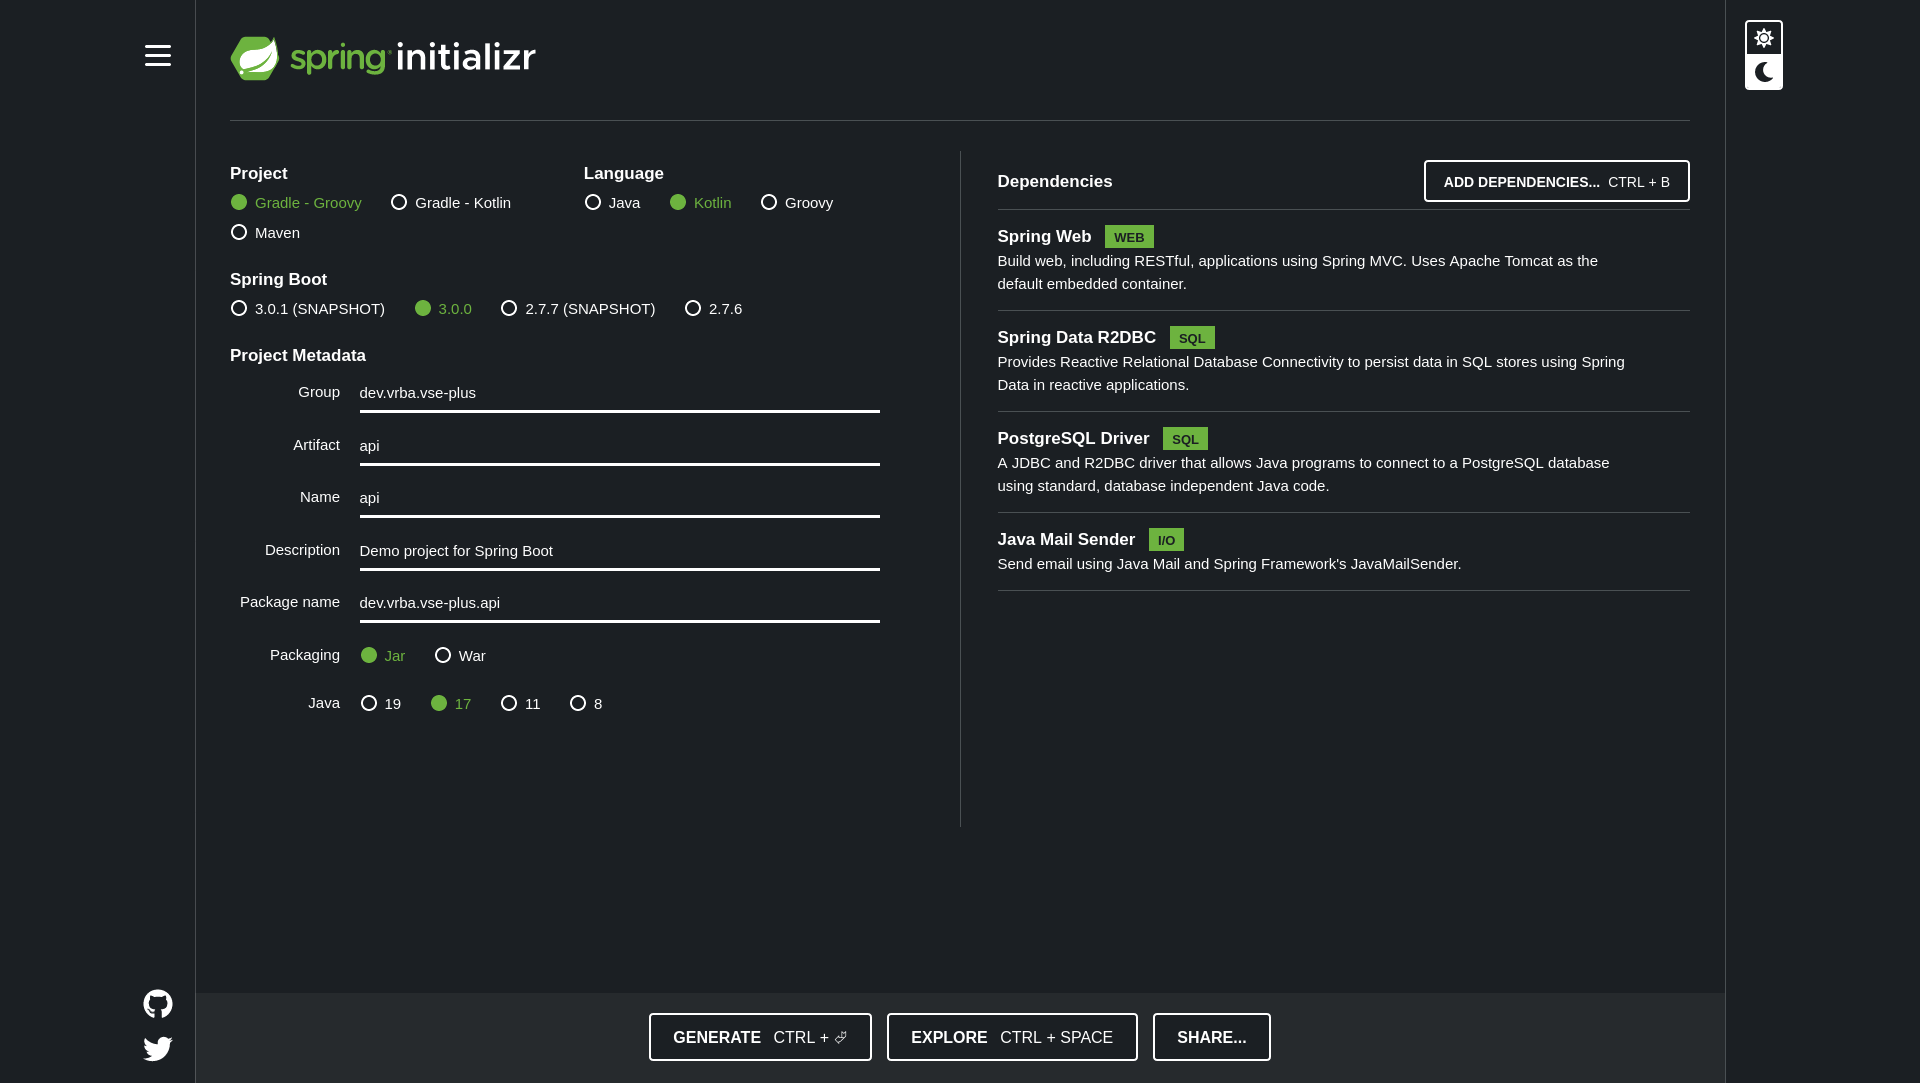
\includegraphics[width=\textwidth]{img/sprint-initializr.png}
\caption{Webové rozhraní nástroje Spring Initializr (vlastní zpracování)}
\label{obr1:SpringInitializr}
\end{figure}

Pro splnění požadavků kladených na funkcionalitu podpůrného serveru vytyčených v~kapitole \ref{sec:pozadavky-na-zvolenou-technologii} je možné použít následující moduly:

\begin{itemize}
    \item \verb|spring-web| pro příjímání a odpovědi na HTTP požadavky,
    \item \verb|spring-json| pro zpracování formátu JSON. Je součástí modulu \verb|spring-web|,
    \item \verb|spring-data| pro ukládání a načítání dat z~relační databáze,
    \item \verb|spring-security| pro autentikaci a autorizaci uživatelů,
    \item \verb|spring-mail| pro odesílání emailů pomocí externího SMTP serveru.
\end{itemize}

\subsubsection{ASP.NET}

ASP.NET je aplikační rámec pro vývoj webových aplikací pomocí technologie .NET vyvinutý společností Microsoft. Podobně jako u~aplikačního rámce Spring se jedná o~platformu, která není omezená pouze na vývoj webových aplikací. Jedná se například o~velice populární platformu vývoj desktopových aplikací pro operační systém Windows.

Aplikační rámec ASP.NET byl poprvé vydán společností Microsoft v~roce 2002 \cite{bekker_microsoft_2002} a jedná se o~zdaleka nejpopulárnější aplikační rámec pro programovací jazyky založené na běhovém prostředí CLR (Common Language Runtime), mezi které patří například programovací jazyk C\# nebo Visual Basic \cite{warren_clr_2022}.

Rámec ASP.NET poskytuje všechny potřebné moduly pro implementaci požadavků kladených na podpůrný webový server. Přímo aplikační rámec ASP.NET má zabudovanou podporu pro příjímání a odpovědi na HTTP požadavky a zpracování formátu JSON \cite{dotnet_web_2023}.

Pro podporu autentikace a autorizace uživatelů má ASP.NET připravenou sadu externích balíčků, které umožňují registrovat schémata pro autentikaci uživatelů a následně definovat přístupová pravidla pro autorizaci uživatelů \cite{dotnet_security_2022}.

\subsubsection{Laravel}

Laravel je webový aplikační rámec vyvinutý pro vývoj webových aplikací v~programovacím jazyce PHP. Programovací jazyk PHP je open source jazyk speciálně navržený pro tvorbu webových aplikací \cite{what_is_php}. Aplikační rámec Laravel poskytuje podporu pro časté požadavky na webové aplikace v~podobě externích balíčků pro práci s~databázovými systémy, autentikace a autorizace uživatelů, zasílání emailů, renderování šablon a další \cite{laravel}. 

Stejně jako předchozí dva zmíněné aplikační rámce, Laravel poskytuje formu abstrakce nad vymezenými funkcionalitami, což umožňuje rychlejší a jednodušší tvorbu aplikací, protože se o~konkrétní funkcionalitu stará přímo aplikační rámec a nikoliv programátor, který tento aplikační rámec využívá.

Jednou z~předností aplikačního rámce Laravel je vysoká rychlost a dynamika při vývoji webových aplikací a krátká zpětnovazební smyčka, což je dobré zejména pro vývoj prototypů výsledného produktu, které můžou být využity pro otestování business modelu a najití potencionálních míst pro zlepšení.

\subsection{Zvolená technologie}

Po zvážení výhod a nevýhod všech zmíněných technologií byl zvolen pro implementaci podpůrného webového serveru aplikační rámec Spring Boot ve spojení s~programovacím jazykem Kotlin, protože nejlépe odpovídal potřebám autora a protože s~programováním serverů v~této kombinaci programovacího jazyka a aplikačního rámce má autor již dlouholetou předchozí zkušenost. Programovací jazyk Kotlin byl zvolen mimo jiné i kvůli jeho výhodám oproti programovacímu jazyku Java, které byly zmíněny v~kapitole \ref{sec:kotlin}.